\documentclass{../../slides-style}

\slidetitle{Введение, многопоточное программирование}{07.09.2023}

\begin{document}

    \begin{frame}[plain]
        \titlepage
    \end{frame}

    \section{Введение}

    \begin{frame}
        \frametitle{О чём этот курс}
        \begin{itemize}
            \item Кратко про почти всё, что обязательно знать любому прикладному программисту
            \begin{itemize}
                \item Многопоточное программирование
                \item Сетевое программирование
                \item Веб-программирование
                \item Работа с базами данных
                \item Рефлексия
            \end{itemize}
            \item Язык программирования --- C\#
        \end{itemize}
    \end{frame}

    \begin{frame}
        \frametitle{Отчётность}
        \begin{itemize}
            \item Домашка
            \item Три контрольные
            \begin{itemize}
                \item Баллы за две лучшие идут в зачёт
                \item Нельзя переписывать (только на зачёте/пересдаче/комиссии)
            \end{itemize}
            \item Доклады (за дополнительные баллы)
            \item Курс на HwProj: \url{http://hwproj.ru/courses/10011}
        \end{itemize}
    \end{frame}

    \begin{frame}
        \frametitle{Критерии оценивания}
        \begin{itemize}
            \item ECTS
            \item Баллы за домашние задачи, баллы за контрольные и даже небольшие баллы за работу в аудитории
            \item Общий балл за домашки: $MAX(0, (n/N – 0.6)) * 2.5 * 100$
            \item Общий балл за контрольные: $n/N * 100$
            \item Итоговая оценка: минимум из этих двух баллов
            \item Дедлайны по домашкам, -1 балл за каждую неделю после дедлайна
            \item Сгорает не более половины баллов
            \item Домашек будет меньше, но они будут больше
        \end{itemize}
    \end{frame}

    \section{Многопоточность, введение}

    \begin{frame}
        \frametitle{Многопоточное программирование}
        Зачем это нужно:
        \begin{itemize}
            \item Оптимально использовать ресурсы процессора
            \begin{itemize}
                \item Одноядерных процессоров практически не бывает
            \end{itemize}
            \item Использовать асинхронные операции ввода-вывода
            \item Не ``вешать'' GUI
        \end{itemize}
        \vspace{5mm}
        Потенциальные проблемы:
        \begin{itemize}
            \item Тысяча способов прострелить себе ногу
            \begin{itemize}
                \item Ошибки могут воспроизводиться раз в тысячу лет и их невозможно обнаружить статически
            \end{itemize}
            \item Не всегда многопоточная программа работает быстрее однопоточной
        \end{itemize}
    \end{frame}

    \begin{frame}
        \frametitle{Процессы и потоки}
        \begin{itemize}
            \item Процесс --- исполняющаяся программа
            \begin{itemize}
                \item Загруженный в память .exe-шник со всеми его .dll-ками или аналогичные понятия
                \item Имеет выделенные для него системные ресурсы:
                \begin{itemize}
                    \item Память
                    \item Открытые файлы
                    \item Открытые сетевые соединения
                    \item ...
                \end{itemize}
            \end{itemize}
            \item Поток --- единица параллельной работы
            \begin{itemize}
                \item Существует внутри процесса
                \item Имеет свой стек и состояние регистров процессора
                \item Все потоки внутри процесса разделяют общие ресурсы (например, память)
            \end{itemize}
        \end{itemize}
    \end{frame}

    \begin{frame}
        \frametitle{Параллельное программирование}
        \begin{itemize}
            \item Параллельная программа может быть:
            \begin{itemize}
                \item Многопроцессной
                \begin{itemize}
                    \item Несколько процессов, возможно, несколько потоков в каждом
                \end{itemize}
                \item Многопоточной
            \end{itemize}
            \item Многопроцессные программы:
            \begin{itemize}
                \item Могут исполняться на разных компьютерах
                \item Пример --- веб-приложения
                \item Сложное и медленное взаимодействие между процессами
            \end{itemize}
            \item Многопоточные программы:
            \begin{itemize}
                \item Могут исполняться только на одном компьютере (нужна общая память)
                \item Быстрое общение между потоками через общую память
                \item Потоки могут портить состояние друг другу
            \end{itemize}
        \end{itemize}
    \end{frame}

    \begin{frame}
        \frametitle{Насколько вообще можно распараллелить}
        \begin{itemize}
            \item Распараллеливание может дать неожиданно низкий прирост производительности
            \item Закон Амдала:
                $$S_p = \frac{1}{\alpha + \frac{1 - \alpha}{p}}$$
            \begin{itemize}
                \item $p$ --- количество процессоров (абстрактных)
                \item $\alpha$ --- доля строго последовательных расчётов
                \item $1 - \alpha$ --- доля расчётов, которые можно идеально распараллелить
                \item $S_p$ --- ускорение
            \end{itemize}
            \item Если у вас есть 9 задач на 1 минуту и 1 задача на 2 минуты, на 10 процессорах ускорение будет всего в 5.5 раз!
            \begin{itemize}
                \item 11 единиц работы, 10 из которых идеально параллельны, одна нет
            \end{itemize}
            \item Добавлять ядра с какого-то момента бессмысленно
        \end{itemize}
    \end{frame}

    \section{Введение в устройство ОС}

    \begin{frame}
        \frametitle{Внезапно, операционные системы}
        Функции операционной системы:
        \begin{itemize}
            \item Предоставлять упрощённый доступ к оборудованию
            \begin{itemize}
                \item Файловая система
                \item Драйвера
            \end{itemize}
            \item Управлять ресурсами компьютера
            \begin{itemize}
                \item Виртуальная память
                \item Планировщик
            \end{itemize}
        \end{itemize}
    \end{frame}

    \begin{frame}
        \frametitle{Планировщик}
        \begin{itemize}
            \item Управляет распределением процессорного времени между процессами и потоками
            \item Каждому потоку выделяется квант времени, прерывание по таймеру
            \item Поток может отдать ядро процессора до истечения кванта
            \begin{itemize}
                \item Сам
                \item Блокирующая операция ввода-вывода
                \item Подгрузка страницы памяти из свопа
                \item Аппаратное прерывание
            \end{itemize}
            \item Хитрые алгоритмы планирования
            \begin{itemize}
                \item Обеспечение максимального быстродействия при справедливом планировании
                \item Учитываются приоритеты потоков
            \end{itemize}
        \end{itemize}
    \end{frame}

    \begin{frame}
        \frametitle{Планировщик в Windows}
        \begin{itemize}
            \item Раз в квант времени (или чаще) выбирает поток для исполнения
            \begin{itemize}
                \item Рассматриваются только потоки, не ждущие чего-либо
            \end{itemize}
            \item НЕ реальное время
            \begin{itemize}
                \item Нельзя делать предположения, когда потоку дадут поработать
            \end{itemize}
            \item Из рассматриваемых потоков выбираются только те, у кого наибольший приоритет
            \begin{itemize}
                \item Приоритеты потоков от 0 до 31, обычно 8
            \end{itemize}
            \item Есть ещё приоритеты процессов: Idle, Below, Normal, Normal, Above Normal, High и Realtime
            \item Относительные приоритеты потоков: Idle, Lowest, Below Normal, Normal, Above Normal, Highest и Time-Critical
            \begin{itemize}
                \item Истинный приоритет получается из относительного приоритета и приоритета процесса
            \end{itemize}
        \end{itemize}
    \end{frame}

    \begin{frame}
        \frametitle{Поток в Windows}
        \begin{itemize}
            \item Thread Kernel Object (\textasciitilde1240 байт)
            \item Thread environment block (TEB) (4 Кб)
            \item User-mode stack (1 Мб)
            \item Kernel-mode stack (24 Кб)
        \end{itemize}

        Ещё для каждой dll-ки, загруженной для процесса при старте или остановке потока, вызывается DllMain с параметрами DLL\_THREAD\_ATTACH и DLL\_THREAD\_DETACH

        \vspace{3mm}
        Квант времени --- \textasciitilde20-30 мс, после чего происходит \textit{переключение контекстов}
    \end{frame}

    \begin{frame}
        \frametitle{Две точки зрения на потоки}
        \begin{itemize}
            \item Поток как абстракция параллельного вычисления --- поток запускается, принимая функцию, которую он должен исполнять
            \begin{itemize}
                \item Долгие вычисления, выполняющиеся независимо от остальных
                \item Слежение за состоянием устройства
                \item Индикация прогресса
            \end{itemize}
            \item Поток как абстракция вычислителя --- поток запускается и готов в бесконечном цикле принимать задачи
            \begin{itemize}
                \item Куча коротких вычислений
                \begin{itemize}
                    \item Потому что запуск потока дорог
                    \item И нет смысла иметь активных потоков больше, чем ядер процессора
                \end{itemize}
                \item Реактивные системы, сетевые соединения и т.д.
            \end{itemize}
        \end{itemize}
    \end{frame}

    \begin{frame}
        \frametitle{Как делать не надо}
        \begin{center}
            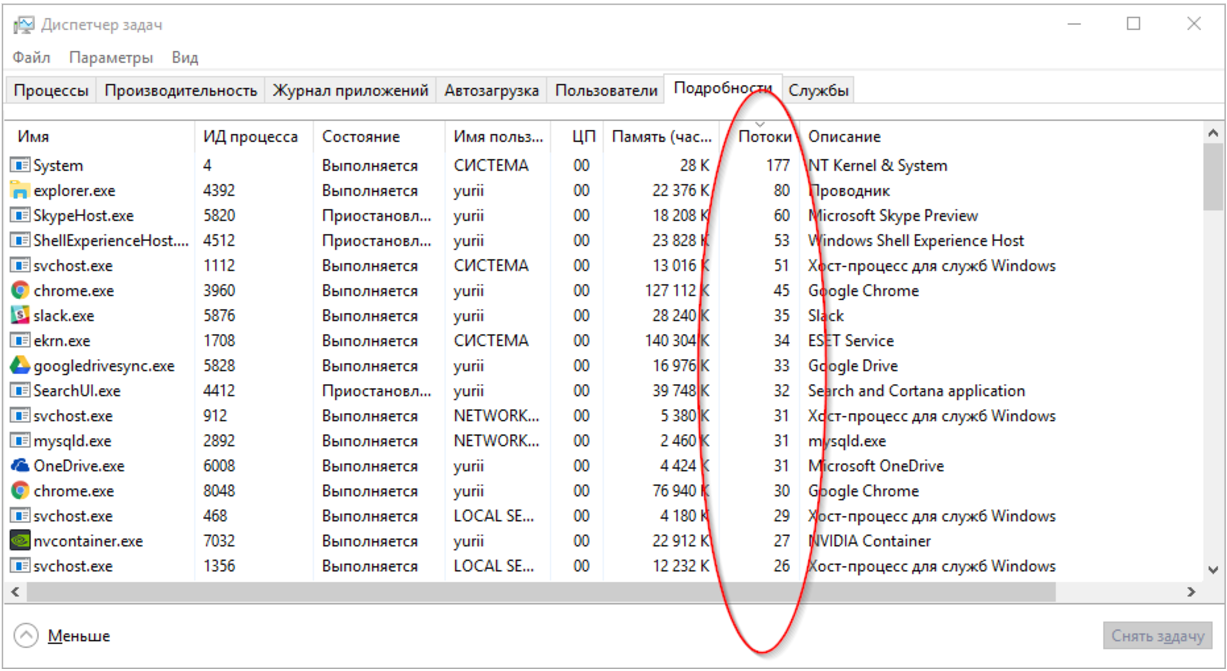
\includegraphics[width=0.9\textwidth]{threadsEverywhere.png}
        \end{center}
    \end{frame}

    \section{Потоки в .NET}

    \begin{frame}[fragile]
        \frametitle{System.Threading.Thread}
        \begin{footnotesize}
            \begin{minted}{csharp}
namespace MultiThreadingDemo;

using System;
using System.Threading;

var otherThread = new Thread(() => {
    while (true)
    {
        Console.WriteLine("Hello from other thread!");
    }
});

otherThread.Start();

while (true)
{
    Console.WriteLine("Hello from this thread!");
}
            \end{minted}
        \end{footnotesize}
    \end{frame}

    \begin{frame}[fragile]
        \frametitle{Параллельная обработка данных}
        \begin{ssmall}
            \begin{minted}{csharp}
using System;
using System.Threading;

var array = new int[] { 1, 5, 2, 4, 7, 2, 4, 9, 3, 6, 5 };
var threads = new Thread[3];
var chunkSize = array.Length / threads.Length + 1;
var results = new int[threads.Length];

for (var i = 0; i < threads.Length; ++i) 
{
    var localI = i;
    threads[i] = new Thread(() => {
        for (var j = localI * chunkSize; j < (localI + 1) * chunkSize && j < array.Length; ++j)
            results[localI] += array[j];
    });
}

foreach (var thread in threads)
    thread.Start();
foreach (var thread in threads)
    thread.Join();

var result = 0;
foreach (var subResult in results)
    result += subResult;

Console.WriteLine($"Result = {result}");
            \end{minted}
        \end{ssmall}
    \end{frame}

    \section{Проблемы синхронизации}

    \begin{frame}[fragile]
        \frametitle{``Упрощённая'' версия}
        \begin{ssmall}
            \begin{minted}{csharp}
using System;
using System.Threading;

var array = new int[] { 1, 5, 2, 4, 7, 2, 4, 9, 3, 6, 5 };
var threads = new Thread[3];
var chunkSize = array.Length / threads.Length + 1;
var result = 0;

for (var i = 0; i < threads.Length; ++i) {
    var localI = i;
    threads[i] = new Thread(() => {
        for (var j = localI * chunkSize; j < (localI + 1) * chunkSize && j < array.Length; ++j)
            result += array[j];
    });
}

foreach (var thread in threads)
    thread.Start();
foreach (var thread in threads)
    thread.Join();

Console.WriteLine($"Result = {result}");
            \end{minted}
        \end{ssmall}
    \end{frame}

    \begin{frame}[fragile]
        \frametitle{Немного увеличим размер задачи...}
        \begin{ssmall}
            \begin{minted}{csharp}
using System;
using System.Threading;

var array = new int[1000];
for (var i = 0; i < array.Length; ++i)
    array[i] = 1;

var threads = new Thread[8];
var chunkSize = array.Length / threads.Length + 1;
var result = 0;

for (var i = 0; i < threads.Length; ++i) {
    var localI = i;
    threads[i] = new Thread(() => {
        for (var j = localI * chunkSize; j < (localI + 1) * chunkSize && j < array.Length; ++j)
            result += array[j];
    });
}

foreach (var thread in threads)
    thread.Start();
foreach (var thread in threads)
    thread.Join();

Console.WriteLine($"Result = {result}");
            \end{minted}
        \end{ssmall}
    \end{frame}

    \begin{frame}[fragile]
        \frametitle{Почему так}
        \mintinline{csharp}|result += array[j];|

        \hspace{13mm}$\Downarrow$

        \begin{ssmall}
            \begin{minted}{text}
IL_0016: ldarg.0      // this
IL_0017: ldfld        class Program/'<>c__DisplayClass0_0' Program/'<>c__DisplayClass0_1'::'CS$<>8__locals1'
IL_001c: ldarg.0      // this
IL_001d: ldfld        class Program/'<>c__DisplayClass0_0' Program/'<>c__DisplayClass0_1'::'CS$<>8__locals1'
IL_0022: ldfld        int32 Program/'<>c__DisplayClass0_0'::result
IL_0027: ldarg.0      // this
IL_0028: ldfld        class Program/'<>c__DisplayClass0_0' Program/'<>c__DisplayClass0_1'::'CS$<>8__locals1'
IL_002d: ldfld        int32[] Program/'<>c__DisplayClass0_0'::'array'
IL_0032: ldloc.0      // j
IL_0033: ldelem.i4    
IL_0034: add          
IL_0035: stfld        int32 Program/'<>c__DisplayClass0_0'::result
            \end{minted}
        \end{ssmall}
        \vspace{5mm}
        Между \textbf{любыми} инструкциями поток может быть прерван
    \end{frame}

    \begin{frame}
        \frametitle{Race condition}
        \begin{center}
            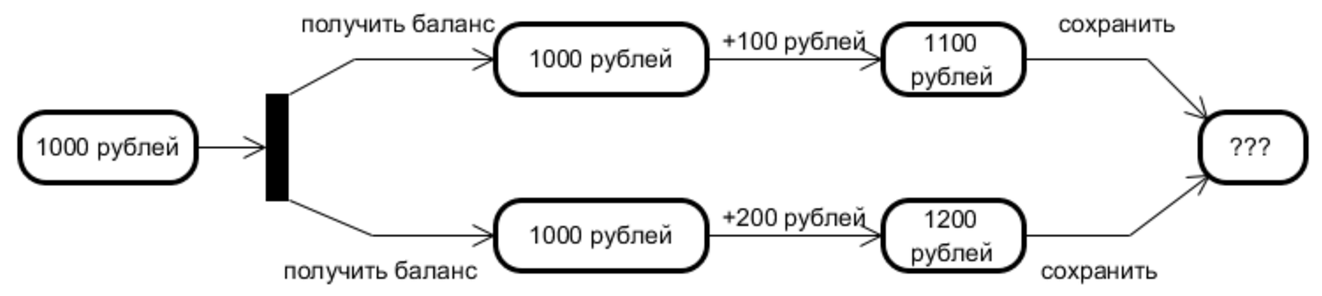
\includegraphics[width=0.9\textwidth]{raceCondition.png}
        \end{center}
    \end{frame}

    \begin{frame}
        \frametitle{Deadlock}
        \begin{center}
            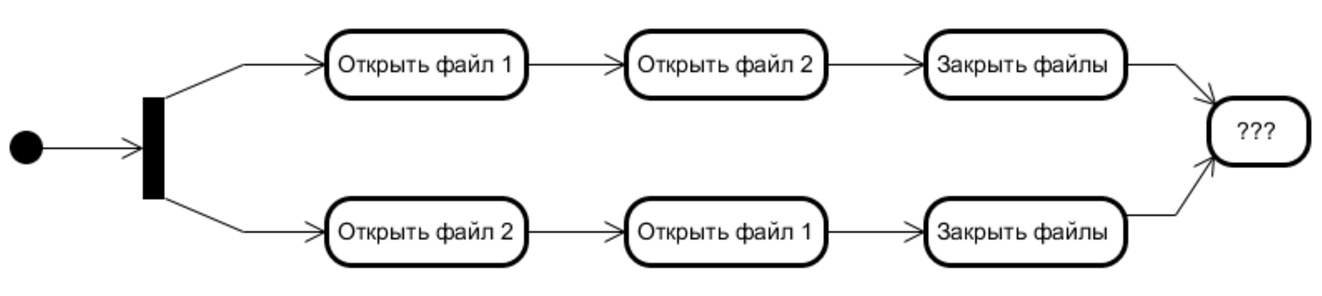
\includegraphics[width=0.9\textwidth]{deadlock.png}
        \end{center}
    \end{frame}
    
    \begin{frame}
        \frametitle{Условия взаимной блокировки}
        \begin{enumerate}
            \item имеется разделяемый ресурс, к которому потоки хотят получить доступ, но пользоваться им может только один поток
            \item таких ресурсов несколько, и поток, захватив один, хочет получить доступ к другим, которые в этот момент захвачены другими потоками
            \item нельзя отнять захваченный ресурс у потока
            \item потоки ждут друг друга <<по кругу>>
        \end{enumerate}
        Блокировка возможна, только если выполнены сразу все эти условия.
    \end{frame}

    \begin{frame}
        \frametitle{Какие ещё ловушки бывают}
        \begin{itemize}
            \item Процессор может переставлять местами инструкции
            \begin{itemize}
                \item Результат исполнения гарантируется таким же, как оригинальный, но промежуточные результаты другим 
                    ядрам могут быть видны странные
            \end{itemize}
            \item У ядер процессора есть кеш (у каждого свой)
            \begin{itemize}
                \item На самом деле, обычно три уровня кеша: L1 и L2 для каждого ядра свой, L3 общий для всех ядер
                \item Кеши синхронизируются, но есть буферы чтения и записи, они нет
            \end{itemize}
        \end{itemize}
    \end{frame}

\end{document}
